% Derived from projects/eos/trunk/ds13.tex.  Another good source might
% be projects/like9501/xcp8_1_14
\documentclass{beamer}
\setbeamertemplate{navigation symbols}{} %no nav symbols
\usepackage{amsmath,amsfonts}
\usepackage[pdftex]{rotating}
\newcommand\logx{y}
\newcommand\logf{g}
\newcommand\Logf{G}
\newcommand{\argmin}{\operatorname*{argmin}}
\newcommand{\La}{{\cal L}}
\newcommand{\C}{{\cal C}}
\newcommand{\normal}[2]{{\cal N}(#1,#2)}
\newcommand{\COST}{\cal C}
\newcommand{\LL}{{\cal L}}
\newcommand{\X}{{\cal X}}
\newcommand{\PS}{{\cal P}}
\newcommand{\Prob}{\text{Prob}}
\newcommand{\field}[1]{\mathbb{#1}}
\newcommand{\EV}[2]{\field{E}_{#1}\left[#2\right]}
\newcommand\inner[2]{\left<#1,#2\right>}
\newcommand{\nomf}{\tilde f}
\newcommand\Polytope[1]{\field{P}_{#1}}
\newcommand\RN{\field{R}^{N}}
\newcommand\PolytopeN{\Polytope{N}}
\newcommand{\T}{{\cal P}}
\newcommand{\partialfixed}[3]{\left. \frac{\partial #1}{\partial #2}\right|_#3}
\newcommand\CJ[1]{{{#1}_{\text{CJ}}}}
\newcommand\dum{\xi}
\newcommand\Ddum{d\dum}

\title{The F\_UNCLE Project: Functional UNcertainty Constrained by Law and Experiment\footnote{LA-UR-17-xxxx}}

\author{Andy Fraser}
\institute{Los Alamos National Laboratory}
\date{2017-2-8}

% \usetheme{Pittsburgh}
\usetheme{default}
\usefonttheme[]{serif}
\begin{document}
\frame{\titlepage
}

\frame{ \frametitle{Outline}\tableofcontents}

\section{Theory: EOS, Isentrope, Shock and Detonation}
\frame{
  \frametitle{Equations of State and Isentropes}

  \begin{columns}
    \begin{column}{0.6\textwidth}
      \resizebox{0.99\textwidth}{!}{\includegraphics{surf.pdf}}
    \end{column}
    \begin{column}{0.4\textwidth}
    \begin{align*}
      pv &= NRT & &\text{Ideal Gas} \\
      pv^3 &\approx c(S) & &\text{For an explosive}
    \end{align*}
    \end{column}
  \end{columns}
}
\frame{
  \frametitle{Shocks, Conservation and Chapman Jouguet Conditions}

  \begin{columns}
    \begin{column}{0.4\textwidth}
      Assumptions:
      \begin{itemize}
      \item 1-d
      \item Instantaneous detonation
      \item Stationary in moving frame
      \item Conserve: Mass, momentum and energy
      \end{itemize}
    \end{column}
    \begin{column}{0.6\textwidth}
      Slope of \emph{Rayleigh line}: $-(\rho_0 D)^2$
      \begin{center}
      \resizebox{0.99\textwidth}{!}{\includegraphics{figs/stick_CJ.pdf}}
        %FixMe: limit v axis
      \end{center}
    \end{column}
  \end{columns}
}

\section{Goals and Experiments}
\frame{
  \frametitle{Goals}
  %
  The stockpile stewardship mission involves simulating detonation
  experiments with multiple shocks.  For such simulations, we need a
  \emph{regional EOS}
  \begin{itemize}
  \item Near nominal \emph{CJ} isentrope
  \item Extension to higher densities
  \item Extension to higher entropies (temperatures)
  \end{itemize}
}
\frame{
  \frametitle{Use Data from Many Experiments}
  \begin{columns}
    \begin{column}{0.4\textwidth}
  \begin{itemize}
  \item Rate sticks
  \item Overdriven flyers
  \item Copper clad cylinders
  \end{itemize}
    \end{column}
    \begin{column}{0.6\textwidth}
      \begin{center}
      \resizebox{0.99\textwidth}{!}{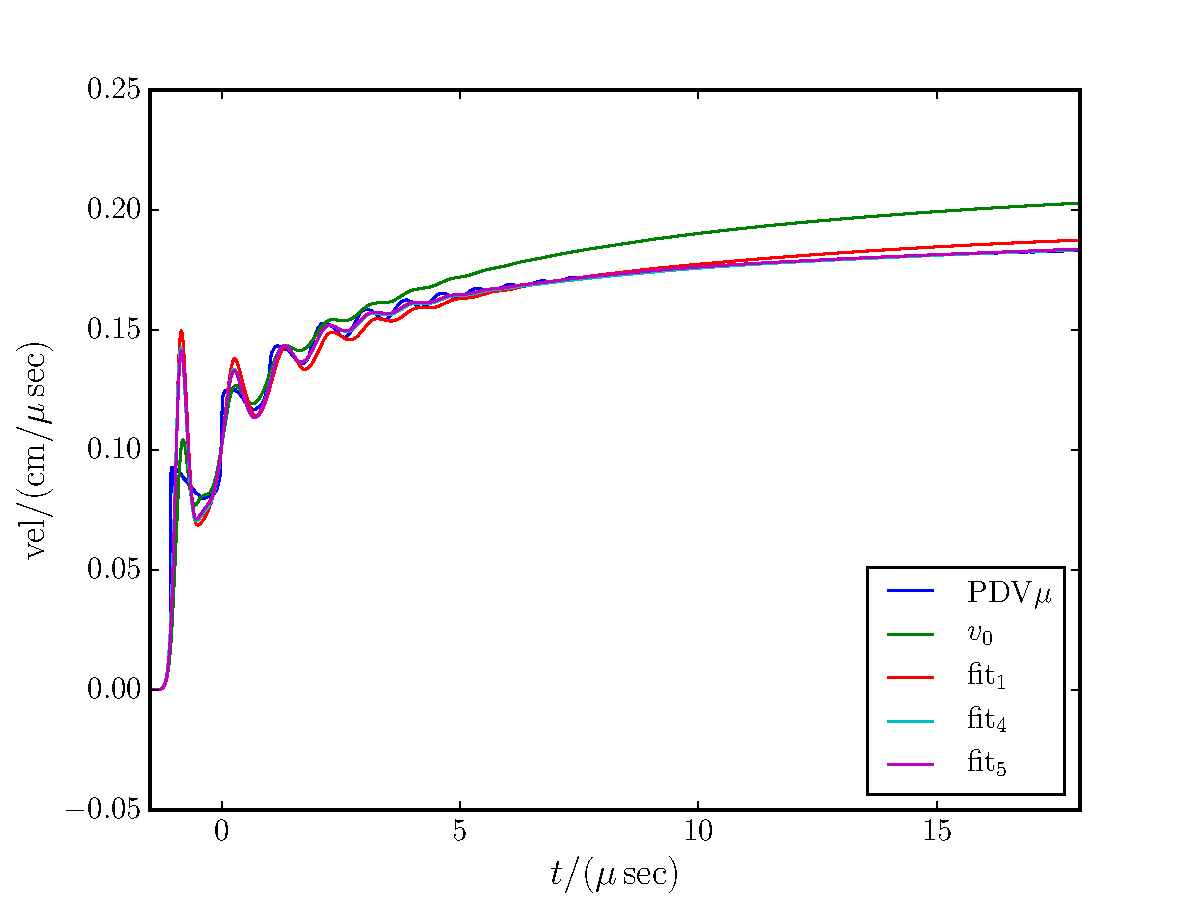
\includegraphics{static_figs/real.pdf}}
        Data and simulations of copper clad cylinders
      \end{center}
    \end{column}
  \end{columns}
}
\section{Analysis: Optimization and Uncertainty}
\frame{
  %
  \frametitle{Mie-Gruneisen form for Empirical EOS}
  %
  Fit two functions of specific volume along nominal \emph{CJ}
  isentrope:
  \begin{description}
  \item[$p(V)$] Pressure
  \item[$\Gamma = V\left( \frac {dp}{de} \right)_V$] Gruneisen gamma.
    Provides states off of the nominal \emph{CJ} isentrope.
  \end{description}
  From now on, I focus on $p(V)$.
}
\frame{
  \frametitle{Constrained Optimization}
  %
  \begin{description}
  \item[Constraints] As a function of volume, pressure must be
    \begin{itemize}
    \item Positive
    \item Monotonic
    \item \textbf{Convex}
    \end{itemize}
  \item[Cost] Weighted sum of squares or
    $C(\theta) = -\log(\text{a posteriori probability})$
  \end{description}
    \begin{align*}
      C(\theta) &= -\frac{1}{2} \sum_i \left(x_i - \mu_i(\theta)
      \right)^T \Sigma_i^{-1} \left(x_i - \mu_i(\theta)
      \right)\\
      &\equiv \sum_i \LL_i  && \text{Log likelihood} \\
      &\quad - \frac{1}{2} \left(\theta - \mu_\theta \right)^T
      \Sigma_\theta^{-1}  \left(\theta - \mu_\theta \right)\\
      &\equiv \LL_0 && \text{Log prior} 
    \end{align*}
}

\frame{
  \frametitle{Surrogate Problem}
  Rate Stick
  \begin{columns}
    \begin{column}{0.5\textwidth}
      \begin{center}
        \resizebox{0.99\textwidth}{!}{
          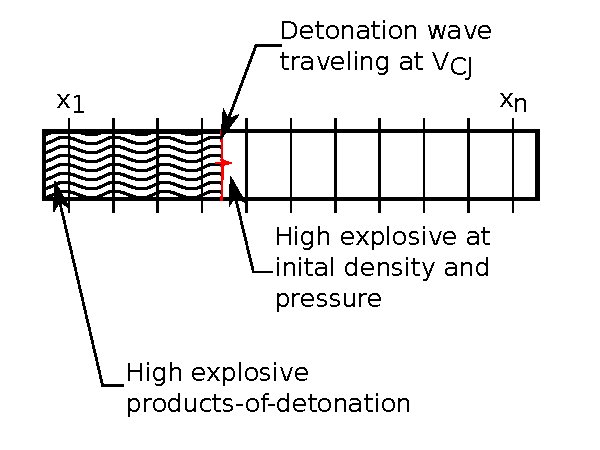
\includegraphics{static_figs/stick_poster.pdf}}
      \end{center}
    \end{column}
    \begin{column}{0.5\textwidth}
      \begin{center}
        \resizebox{0.99\textwidth}{!}{\includegraphics{figs/stick_xt.pdf}}
      \end{center}
    \end{column}
  \end{columns}
}

\frame{
  \frametitle{Surrogate Problem Cont.}
  Gun
  \begin{columns}
    \begin{column}{0.5\textwidth}
      \begin{center}
        \resizebox{0.99\textwidth}{!}{
          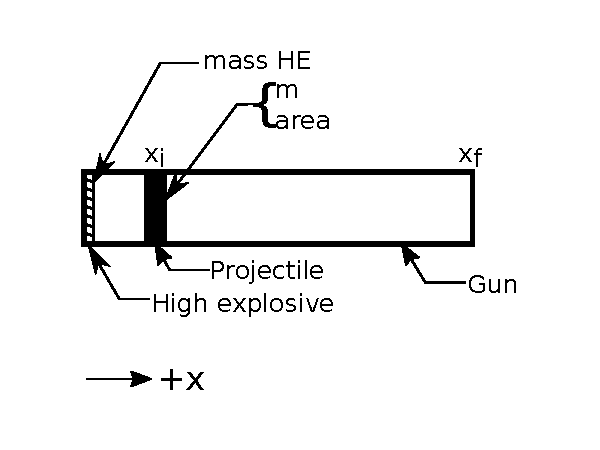
\includegraphics{static_figs/gun_poster.pdf}}
      \end{center}
    \end{column}
    \begin{column}{0.5\textwidth}
      \begin{center}
        \resizebox{0.99\textwidth}{!}{\includegraphics{figs/gun_tv.pdf}}
      \end{center}
    \end{column}
  \end{columns}
}

\frame{
  \frametitle{Uncertainty and Fisher Information}
  After finding $\hat \theta \equiv \argmin_\theta C(\theta)$,
  characterize uncertainty by $\frac{\partial^2}{\partial \theta^2}
  C(\theta)$ or its expected value.  Note:
  \newcommand{\dmudtheta}{\left(\frac{\partial \mu_i(\theta)}
      {\partial \theta} \right)}
  \begin{equation*}
    \frac{\partial^2}{\partial \theta^2} \LL_i(\theta) = 
      \dmudtheta^T \Sigma_i^{-1} \dmudtheta +  (x_i-\mu_i(\theta))^T \Sigma_i^{-1}
       \left(\frac{\partial^2 \mu_i(\theta)}{\partial \theta^2} \right)
  \end{equation*}
  Note: Since $X_i\sim$ symmetric about $\mu_i(\theta)$, the expected
  value of the second term is 0.  The first term called the
  \emph{Fisher Information}
  \begin{equation*}
    {\cal{I}}_i \equiv \EV{x}{\frac{\partial^2}{\partial \theta^2}
      \LL_i} = \dmudtheta^T \Sigma_i^{-1} \dmudtheta
  \end{equation*}
  characterizes how tightly the experiment constrains $\theta$.
}

\frame{
  \frametitle{Fisher Information for the Surrogate Problem}
  Rate Stick
  \begin{columns}
    \begin{column}{0.5\textwidth}
      \begin{center}
        \resizebox{0.99\textwidth}{!}{
          \includegraphics{figs/stick_fisher.pdf}}
      \end{center}
    \end{column}
    \begin{column}{0.5\textwidth}
      Gun
      \begin{center}
        \resizebox{0.99\textwidth}{!}{\includegraphics{figs/gun_fisher.pdf}}
      \end{center}
    \end{column}
  \end{columns}
}

\frame{
  \frametitle{Software}
  We are using F\_UNCLE to learn and demonstrate \emph{Best Practices
    for Scientific Software}.  We use the following tools:
  \begin{itemize}
  \item Python, SciPy, NumPy, CVXOPT
  \item Git
  \item TravisCI
  \item Nosetests
  \item Sphinx
  \end{itemize}
}

\frame{
  \frametitle{The End}
}

\frame{ \frametitle{Abstract}
  %
  We are fitting equations of state (EOS) to the mixtures of gasses
  produced by detonating explosives.  Given a set of experimental
  measurements, we intend our code to provide: 1. An estimate of the
  EOS; 2. A characterization the residual uncertainty. 3. A
  description of how each different experiment (both those that have
  been run and those that are proposed) constrains the estimated EOS.
  Matrices called the \emph{Fisher Information} represent the
  constraints.  The presentation will outline the problem and
  illustrate the resulting constraints.
%
}

\frame{
  \frametitle{Extra Stuff}
      \resizebox{0.8\textwidth}{!}{\includegraphics{figs/eos_nom_true.pdf}}
}

\end{document}

%%%---------------
%%% Local Variables:
%%% eval: (TeX-PDF-mode)
%%% End:
